% !TEX root = ../../main.tex
% !TEX encoding = UTF-8 Unicode
\chapter{The Large Hadron Collider}
\label{ch:lhc}

The Large Hadron Collider (LHC)~\cite{LHC,LHC_design_v1,LHC_design_v2,LHC_design_v3} is a circular particle accelerator designed to probe physics at the \TeV\,scale. By colliding protons or heavy-ions with high energy, at a high rate, in compact beams, the LHC provides access to extremely rare phenomena that have escaped previous experimental efforts. Currently producing the highest energy collisions in the world, the LHC has two rings carrying hadrons in opposite directions around a 26.7\,km loop, with superconducting magnets to bend the particles' trajectories. 

The tunnel housing the accelerator was already built between 1984-1989 for the previous Large Electron-Positron collider (LEP)~\cite{LEP} and is located  at the European Organization for Nuclear Research (CERN) on the border between France and Switzerland, near Geneva, between 45\,m and 170\,m underground. After ten years of construction between 1998-2008, 
%and minor archeology\footnote{Gallo-Roman ruins were unearthed as the Compact Muon Solenoid (CMS) began excavation at their future detector site in July 1998~\cite{lhc_timeline}.},
the LHC began operations in September 2008. Shortly after, a faulty electrical connection between two superconducting magnets caused severe damage and required 14 months of repairs~\cite{lhc_incident}.
% created an arc that damaged the helium coolant enclosure, explosively releasing over 6 tonnes of liquid helium which caused severe damage to 53 superconducting magnets and the vacuum beam pipes as its vapors rapidly expanded in the tunnel~\cite{lhc_incident}. After 14 months of repairs,
The LHC successfully reinitiated operations for Run-I (2010-2012) while operating at a center-of-mass energy $\sqs=7-8$\,\TeV.
%\footnote{In order to ``train'' the superconducting magnets to handle the extremely large currents without ``quenching'', or loosing it's superconducting properties, the magnets are repeatedly run with lower currents to incite smaller quenches, allowing the magnets to slowly ``settle''. It was decided, then, to use lower energy collisions during Run-I to prevent further setbacks.}
Following two years of scheduled upgrades and repairs, the LHC began the current phase, Run-II (2015-2018), where it is operating near the design energy at $\sqs=13$\,\TeV. The data in this thesis was collected during the first two years of Run-II (2015 and 2016). The following chapter will discuss the basic physics involved in the accelerator (\Sect{\ref{ch:lhc:acc}}), the layout and injection chain (\Sect{\ref{ch:lhc:inj}}), the machine design (\Sect{\ref{ch:lhc:des}}), and the participating experiments (\Sect{\ref{ch:lhc:exp}}).

%
\section{Accelerator Physics}
\label{ch:lhc:acc}
With the goal of studying exceedingly rare processes, two parameters can be of particular interest: the center-of-mass energy of the collision, and the frequency of collisions. The LHC addresses both of these concerns. However, each parameter has limiting factors which constrain the design. 

A charged particle in a magnetic field has momentum defined by~\Eqn{\ref{eqn:mag_field}} and will travel in a circular trajectory in the plane perpendicular to the field~\cite{accelerators} . For a circular accelerator of fixed radius, the magnetic field determines the maximum allowed particle momentum. The LHC used the existing LEP tunnel and invested in developing and implementing strong superconducting magnet technology. Since the LHC uses two beams circulating in opposite directions, the upper limit of the center-of-mass energy is the sum of the two beam energies. 
\begin{equation}
p[\textrm{TeV}] =0.3B[\textrm{T}]\cdot R[\textrm{km}] 
\label{eqn:mag_field}
\end{equation}


Besides the limitations on beam energy from size and magnet strength, charged particles that experience acceleration perpendicular to their velocity, such as moving in a circular orbit, lose energy to synchrotron radiation. The power radiated due to synchrotron radiation is shown in~\Eqn{\ref{eqn:synchrotron_rad}}. The power radiated is proportional to $m^{-4}$; thus, heavy particles like protons are much less affected by synchrotron radiation than lighter particles like, for example, electrons. Using the nominal LHC parameters, this translates to each proton losing approximately 10\,\keV\,per turn. 
\begin{equation}
P = \frac{e^2}{6\pi\epsilon_0c^7r^2m^4}E^4
\label{eqn:synchrotron_rad}
\end{equation}


To study rare processes, it is also important to generate many events. The number of expected events, $N_{\textrm{exp}}$, for a process with cross section, $\sigma_{\textrm{exp}}$, is defined by~\Eqn{\ref{eqn:n_evts}} where $\mathcal{L}$ is the instantaneous luminosity, $N_b$ is the number of particles per bunch, $n_b$ is the number of bunches per beam, $f_{\textrm rev}$ is the revolution frequency, and A is the transverse beam area. Generating many collisions, then, can be accomplished by increasing the luminosity, and running the experiment over a long time period.
\begin{equation}
N_{\textrm{exp}} = \sigma_{\textrm{exp}}\int\mathcal{L}(t)dt = \sigma_{\textrm{exp}}\int \frac{N_b^2n_b^2f_{\textrm{rev}}}{A} dt
\label{eqn:n_evts}
\end{equation}

Besides the bending dipole magnets of the LHC, quadrupole magnets are used to produce ``strong focusing'' of the beam: sections that focus the horizontal beam direction and defocus the vertical beam direction alternate with sections that defocus the horizontal beam direction and focus the vertical beam direction. This alternate-gradient focusing has the net effect of focusing the beam in both transverse directions, and allows the beam to reach much higher intensities. However, the focusing also induces betatron oscillations, $\beta(s)$, about a nominal trajectory $s$. For an approximately Gaussian beam, the RMS of the beam size in the transverse direction is $\sigma(s)$. The value of $\beta(s)$ and $\sigma(s)$ measured at the interaction point (IP) is denoted $\beta^*$ and $\sigma^*$ respectively. A measure of the beam spread in position and momentum space, known as transverse emittance $\epsilon$, is defined in~\Eqn{\ref{eqn:trans_emit}}. As emittance scales with energy, an invariant, normalized emittance is defined by $\epsilon_n\equiv \beta_r\gamma_r\epsilon$ where $\beta_r, \gamma_r$ are the relativistic functions. Since the beams do not collide head-on, but rather with a crossing angle $\theta_c$, a geometric factor, $F$, accounting for the corresponding reduction in luminosity is defined in~\Eqn{\ref{eqn:f_fact}}, where $\sigma_z$ is the RMS bunch length. 
\begin{eqnarray}
\epsilon&\equiv& \pi\frac{\sigma^2(s)}{\beta(s)} \label{eqn:trans_emit} \\
F &\equiv& \left[ 1+ \left(\frac{\theta_c\sigma_z}{2\sigma^{*}} \right) \right]^{-1/2} \label{eqn:f_fact} 
\end{eqnarray}
%The nominal values for the LHC for F = 0.78
%Design values: $\theta_c=285\,\mu$rad, $\sigma_z=7.55$\,cm, $\sigma^{*}=16.6\,\mu$m, $\epsilon_n\simeq 3.75\,\mu$m, and $\beta^{*}=0.55\,$m. 
%\footnote{The value of the betatron oscillation function, $\beta(s)$, at the IP is denoted by $\beta^{*}$.}

Using these parameters, the luminosity at the IP from~\Eqn{\ref{eqn:n_evts}} can be expressed as shown in~\Eqn{\ref{eqn:inst_lumi}}.  
%\footnote{$$F = \left[ 1+ \left(\frac{\theta_c\sigma_z}{2\sigma^{*}} \right) \right]^{-1/2}$$ where $\theta_c$ is the full crossing angle at the interaction point (IP), $\sigma_z$ is the RMS bunch length, and $\sigma^{*}$ is the transverse RMS beam size at the IP~\cite{LHC}. Design values: $\theta_c=285\,\mu$rad, $\sigma_z=7.55$\,cm, $\sigma^{*}=16.6\,\mu$m.}
Maximizing the luminosity involves maximizing the beam current, $N_bn_bf_{\textrm{rev}}$, maximizing the beam brightness, $N_b/\epsilon_n$, maximizing the beam energy, and minimizing $\beta^{*}$. Several issues arise and limit the maximum achievable luminosity, including beam-beam effects, space-charge, and limited cryogenic absorption.
\begin{equation}
\mathcal{L} = \frac{N_b^2n_bf_{\textrm{rev}}\gamma_r}{4\pi\epsilon_n\beta^{*}}F(\theta_c,\sigma_z,\beta^{*},\epsilon_n) = \frac{1}{4\pi}\left(N_bn_bf_{\textrm{rev}}\right)\frac{N_b}{\epsilon_n}\frac{\gamma_r}{\beta^{*}}F(\theta_c,\sigma_z,\beta^{*},\epsilon_n)
\label{eqn:inst_lumi}
\end{equation}

In the LHC, due to large uncertainties in determining $\beta^{*}$, the luminosity is not directly measured from the parameters listed in~\Eqn{\ref{eqn:inst_lumi}}; instead, van der Meer scans~\cite{vanderMeer} are used to measure the absolute luminosity during special calibrating runs. A van der Meer scan involves moving the beams relative to each other in both the horizontal and vertical directions while measuring how the event rate changes. The luminosity is rewritten in~\Eqn{\ref{eqn:inel_lumi}} in terms of inelastic collisions, where $\mu = \langle N_{\textrm{inel}}/n_b\rangle$ is the average number of inelastic interactions per bunch crossing. Relative luminosity measurements can be calibrated by measuring the inelastic rate, $R_{\textrm{inel}}$, while the absolute luminosity is determined during a van der Meer scan.
\begin{equation}
\mathcal{L} = \frac{R_{\textrm{inel}}}{\sigma_{\textrm{inel}}} = \frac{\mu n_b f_{rev}}{\sigma_{\textrm{inel}}}
\label{eqn:inel_lumi}
\end{equation}

%
\section{Injection Chain}
\label{ch:lhc:inj}
To accelerate protons into highly focused, stable bunches, a series of injection stages comprised of previous accelerators at CERN is utilized. The full accelerator complex is shown in~\Fig{\ref{fig:lhc_acc_comp}}, including several experiments not associated with the LHC.

The first stage of the injection chain involves producing protons from diatomic hydrogen gas using a metal cylinder, called a Duoplasmatron, in an electric field~\cite{lhc_closer_look}. 
The 100\,\keV\,plasma beam of bare protons leaving the Duoplasmatron is then accelerated up to 750\,\keV\, in the Radio-Frequency Quadrupole (RFQ).
%The gas undergoes a chemical reaction, shown in~\Eqn{\ref{eq:proton_strip}}, producing a  100\,\keV\,plasma beam with bare protons at a 70\% efficiency.
%\footnote{At STP, a typical 5\,kg tank of H$_2$ has 2,500 moles of gas. Assuming a typical LHC beam lifetime of 10 hours, this tank would last: \begin{eqnarray} & 0.7\,(\text{efficiency})\times2500\,\text{mol} \times \frac{6\cdot 10^{23}\,\text{H}_2\,\text{molecules}}{\text{mol}}\times\frac{2\,p^+}{\text{H}_2\,\text{molecule}}\times\frac{\text{bunch}}{1.15\cdot10^{11}\,p^+}\nonumber\\ &\times\frac{\text{run}}{2\times2808\,\text{bunches}}\times\frac{10\,\text{hr}}{\text{run}}\times\frac{\text{yr}}{24\times365.25\,\text{hr}} = 3.7\cdot10^9\,\text{yr}\nonumber\end{eqnarray}} 
%\begin{eqnarray}H_2+e^-&\ra& H_2^+ +2e^- \nonumber\\H_2^+ + e^- &\ra& H^+ + H + e^-\nonumber\\H+e^-&\ra& H^+ + 2e^- \label{eq:proton_strip}\end{eqnarray}
Besides providing acceleration, the RFQ also efficiently focuses and bunches the initially continuous input beam. The next leg of the journey is through the Linear Accelerator 2 (Linac2), whose 200 \,MHz radio-frequency (RF) cavities accelerate the proton bunches to 50\,\MeV\,over 30\,m, while quadrupole magnets keep the beam focused. The protons are transported through 80\,m of connecting pipe, with 20 focusing quadrupole magnets, to the Proton Synchrotron Booster (PSB). In the 25\,m radius PSB, four superimposed rings accelerate the protons further to 1.4\,\GeV\,before injection into the Proton Synchrotron (PS). The high beam brightness, $N_b/\epsilon_n$, has a de-focusing effect due to high space charge\footnote{
	The protons feel an electrostatic repulsion to each other from their charge, but also feel an attraction since they behave like parallel currents as they orbit. For low momenta the repulsion dominates and has a defocussing effect, while in the ultra-relativistic limit the forces cancel.
}; thus, the PSB injects the PS with multiple cycles, lowering $N_b$ per injection, and thus minimizing the impact of space charge. Protons travel around the 628\,m circumference PS for 3.6 seconds, at which point they have been accelerated to 25\,\GeV. In the PS, the proton bunches form trains where each bunch of approximately $1.15\times10^{11}$ protons is separated by 25\,ns. Typically three or four bunch trains are then injected into the 7\,km circumference Super Proton Synchrotron (SPS). The SPS accelerates the bunch trains to 450\,\GeV\, and then injects them into both rings of the LHC. Typically 12 cycles are required to fill each ring in the LHC with the nominal 2,808 bunches. 
\begin{figure}[tbp]
\begin{center}
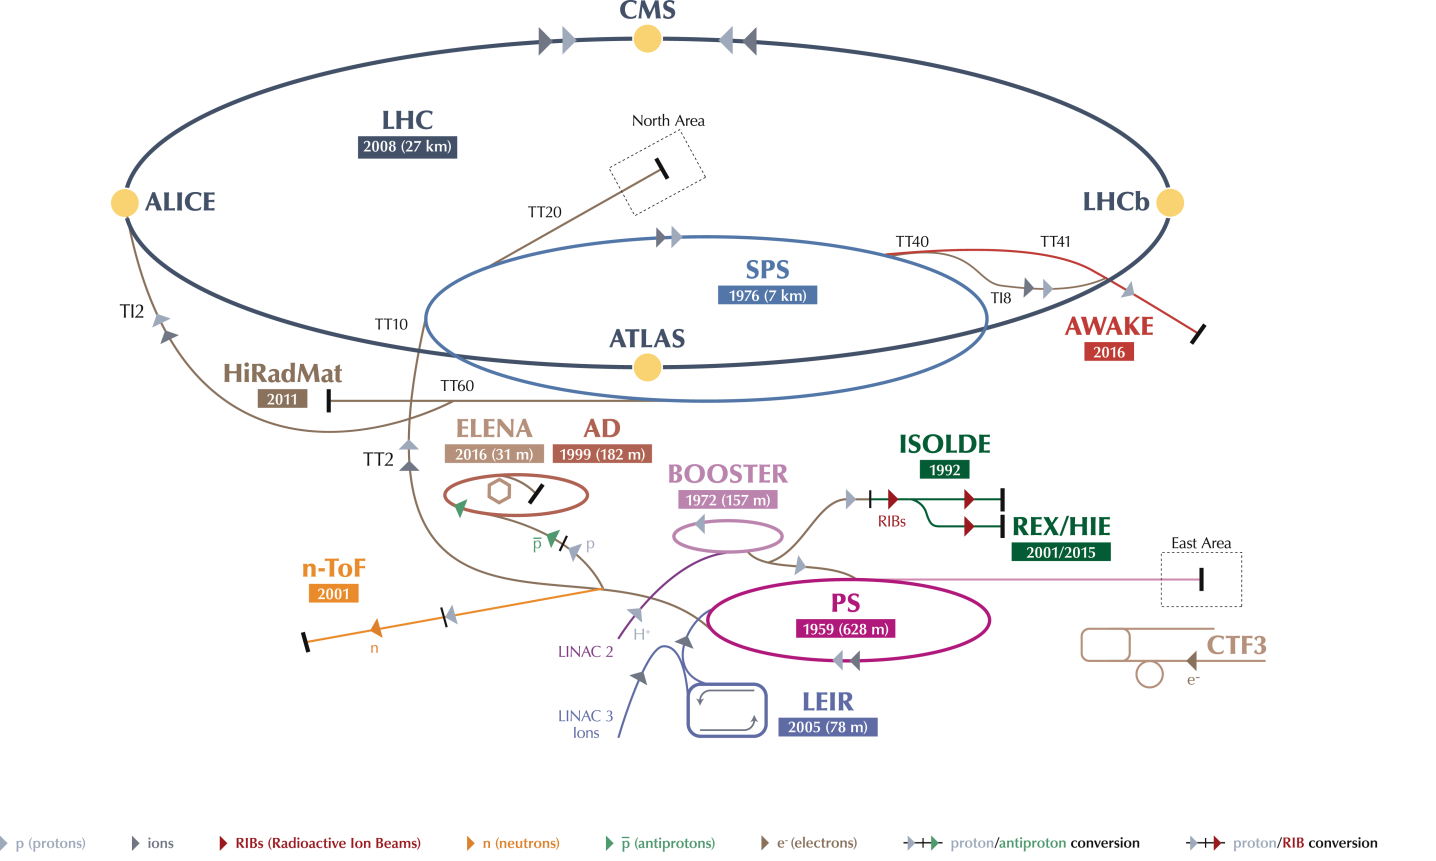
\includegraphics[width=.8\textwidth]{figures/LHC/accelerator}
\end{center}
\caption[The LHC accelerator complex]{The layout of the accelerator complex at CERN. The protons are accelerated through Linac 2, PSB, PS and SPS and then injected into the LHC as shown. Several additional experiments unrelated to the LHC are also depicted~\cite{acc_comp}.}
\label{fig:lhc_acc_comp}
\end{figure}


%
\section{LHC Design}
\label{ch:lhc:des}
The fundamental components of the LHC are the two rings, dipole bending magnets, quadrupole focusing magnets, and RF acceleration cavities. Since the diameter of the LHC tunnel is only 3.7\,m, there is no room for two separate rings. Instead, a ``twin-bore'' dipole magnet design is implemented, whereby both coils and beam channels are magnetically and mechanically coupled inside the same cryostat. 

There are 1,232 superconducting dipole magnets which principally provide the necessary bending for protons circling the LHC. The dipoles consist of coils of superconducting niobium-titanium (NbTi) in two layers around the beam pipe. The wires are arranged so that the current flows in opposite directions on either side of the beam pipe in order to produce a magnetic field perpendicular to the beam line.
%, as depicted in~\Fig{\ref{fig:lhc_magnets}}.
The dipole coils are cooled with superfluid helium to 1.9\,K, well below the critical temperature of the wires, carrying an enormous 11.85\,kA current and producing an 8.33\,T magnetic field. Since the wires on either side of the beam pipe carry currents in opposing directions, they feel a strong repulsive force. Therefore, non-magnetic collars envelop the coils and prevent them from separating. As mentioned previously, the LHC uses quadrupole magnets in an alternate-gradient focusing scheme to constrain the transverse beam profile in both the horizontal and vertical directions.
%, as depicted in~\Fig{\ref{fig:lhc_magnets}}. 
There are 392 such quadrupole magnets interspaced with the dipole magnets and several other, higher multipole adjustment magnets. 
%\begin{figure}
%\begin{center}
%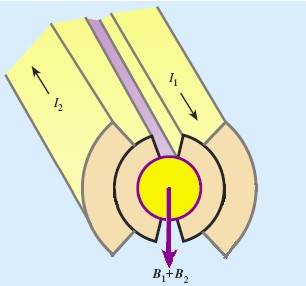
\includegraphics[width=.39\textwidth]{figures/LHC/dipole_bend}
%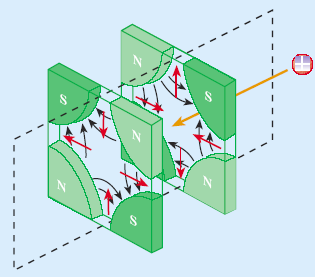
\includegraphics[width=.41\textwidth]{figures/LHC/quad_field}
%\caption[Dipole and quadrupole LHC magnets]{The wires of the dipole magnets (left) are arranged so the current flows in opposite directions on either side of the beam pipe, producing a perpendicular magnetic field. The quadrupole magnet (right) alternate-gradient focusing scheme results in focusing both horizontal and vertical beam profiles~\cite{lhc_closer_look}.}
%\label{fig:lhc_magnets}
%\end{center}
%\end{figure}

In order to accelerate the injected protons to their nominal energy, eight superconducting RF cavities are used per beam. The RF cavities operate at 400\,MHz, generating an oscillating electric field that provides additional kicks to synchronous protons. A proton arriving slightly before or after a synchronous proton will undergo a longitudinal oscillation about the nominal trajectory. This effectively creates RF ``buckets'' in which the LHC bunches are confined. The nominal LHC bunch spacing is 25\,ns, which corresponds to 10 RF buckets. Each RF cavity is made out of a niobium film on a copper cavity, cooled to 4.5\,K. The cavities each deliver 2\,MV, corresponding to a boost per proton of 16\,\MeV\, per turn. 

After both rings of the LHC are filled, the bunches are slowly accelerated, or ``ramped'', over approximately 20 minutes to the nominal collision energy by the RF cavities. When the beams are fully prepared, they are aligned onto each other to provide collisions
%\footnote{Since the LHC is 26.7\,km in circumference, with 25\,ns bunch spacing there is room for 3,550 bunches; however, only 2808 are filled to help with beam injection and dumping. At 6.5\,\TeV, protons have an ultra-relativistic $\gamma_r=6,927$ corresponding to 11,245 trips around the LHC per second. The 2808 bunches thus produce an average crossing rate of 31.6\,MHz. An average interaction per crossing, $\mu$, of $\sim25$ yields $0.8\times10^9$\, collisions per second.} 
at several interaction points around the ring. Further fine-tuning adjustments are made, if required, and then the beams are declared ``stable''. During stable beams, the detectors begin recording the collision data for physics analysis. The beam lifetime is approximately 10\,hours, after which the bunches are dumped and the injection process begins again. 

During an LHC run, the instantaneous luminosity drops as a function of time as the bunches slowly deplete from collisions; therefore, short segments called luminosity blocks are used to estimate periods of approximately equal instantaneous luminosity. Typically, luminosity blocks are around one to two minutes long. Using the instantaneous luminosity measurements for each luminosity block the total integrated luminosity can be calculated. The total luminosity delivered and recorded by ATLAS in 2015 and 2016 is shown in~\Fig{\ref{fig:lumi_2015_2016}}.

\begin{figure}[htbp]
\begin{center}
\includegraphics[width=.49\textwidth]{figures/Atlas/Lumi_2015}
\includegraphics[width=.49\textwidth]{figures/Atlas/Lumi_2016}
\end{center}
\caption[Delivered and recorded luminosity in 2015 and 2016]{The total integrated luminosity versus time delivered to ATLAS (green) and recorded by ATLAS (yellow) during stable beams for $pp$ collisions at $\sqrt{s}=13$\,\TeV\, is shown for 2015 (left) and 2016 (right)~\cite{Lumi_Public_Run2}.}
\label{fig:lumi_2015_2016}
\end{figure}

%
%\clearpage
\section{Experiments at the LHC}
\label{ch:lhc:exp}
%\begin{figure}[htbp]
%\begin{wrapfigure}{r}{.5\textwidth}
%\begin{center}
%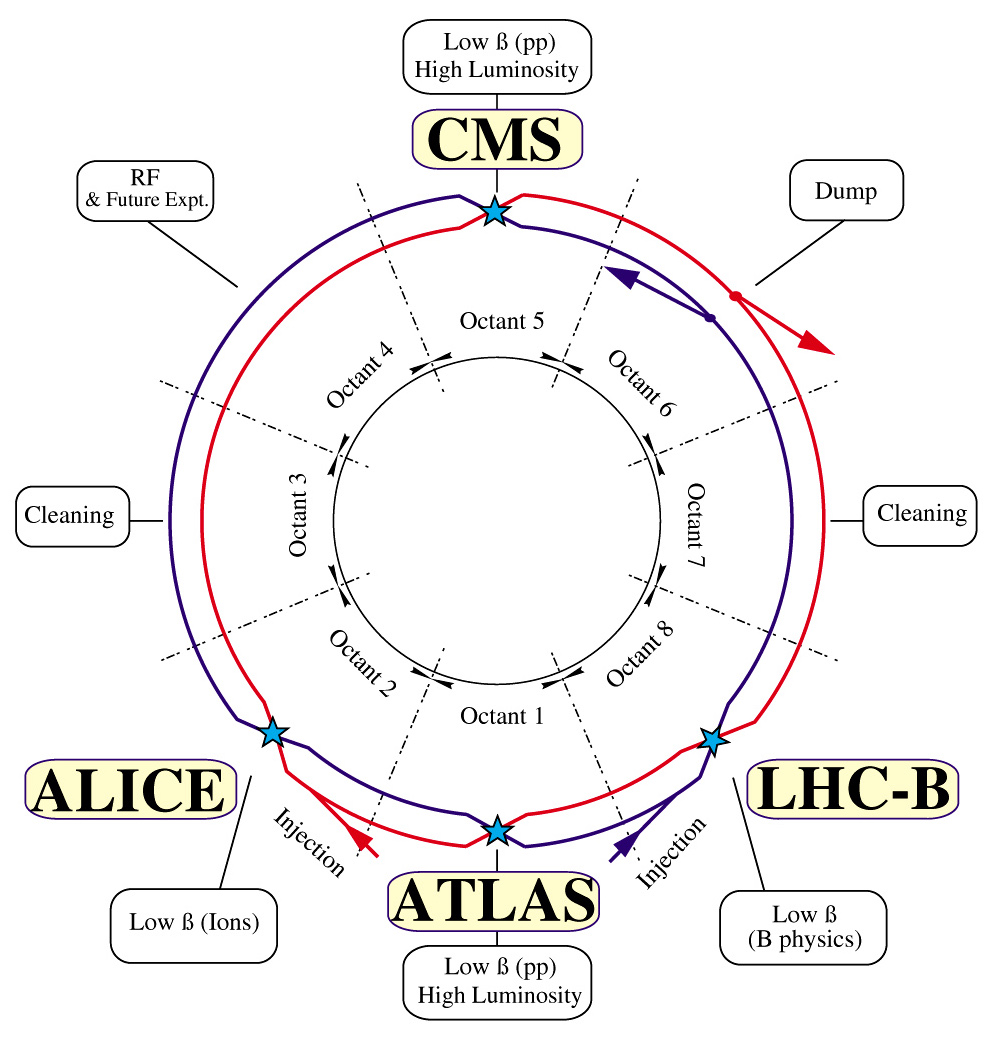
\includegraphics[width=0.49\textwidth]{figures/LHC/lhc-grid}
%\caption[Octant geometry of the LHC]{A schematic of the octant geometry of the LHC: ATLAS and CMS sit opposite each other at Point 1 and Point 5, respectively, while ALICE and LHCb sit adjacent to ATLAS at Point 2 and Point 8, respectively~\cite{LHC}.}
%\label{fig:lhc_grid}
%\end{center}
%\end{wrapfigure}
%\end{figure}
The LHC is constructed with an octant geometry,
%, shown in~\Fig{\ref{fig:lhc_grid}}, 
with eight arcing sections alternating with eight 528\,m straight sections. In the straight sections, the two beams are either brought together at an IP for a detector to measure collisions, or the section are used for services and utilities. There are four main experiments at the LHC: two general-purpose, high-luminosity detectors ATLAS (A Toroidal LHC ApparatuS)~\cite{ATLAS} and CMS (Compact Muon Solenoid)~\cite{CMS}, and two specialized detectors designed for specific phenomena ALICE (A Large Ion Collider Experiment)~\cite{ALICE} and LHCb (Large Hadron Collider beauty)~\cite{LHCb}. The two high-luminosity experiments are placed on opposite sides of the ring: ATLAS is located at Point 1, while CMS is located at Point 5. ALICE and LHCb sit on either side of ATLAS at Point 2 and Point 8, respectively. Both ATLAS and CMS search for a wide spectrum of physics processes. Consequently, the two independently designed experiments offer a valuable cross check in the event of potential discoveries, as was the case with the discovery of the Higgs boson in 2012~\cite{Higgs_atlas,Higgs_cms}. In addition to the four main experiments, three smaller experiments are placed near existing IPs: TOTEM (TOTal Elastic and diffractive cross section Measurement)~\cite{TOTEM}, MoEDAL (Monopole and Exotics Detector at the LHC)~\cite{MoEDAL}, and LHCf (Large Hadron Collider forward)~\cite{LHCf} sit close to CMS, LHCb, and ATLAS respectively. This analysis uses data collected with ATLAS, described in depth in~\Ch{\ref{ch:atlas}}.

%%%
\iffalse
%%%
One of the main design differences between ATLAS and CMS is the magnet system: CMS is designed around a large solenoid magnet that produces a 4\,T field. From IP outwards, the detector consists of a silicon tracker, a scintillating lead tungstate electromagnetic calorimeter, a sampling, plastic-scintillator hadronic calorimeter, a large superconducting solenoid magnet, and a variety  of muon detectors.

Unlike CMS and ATLAS, ALICE is specifically designed to study heavy-ion (Pb-Pb) collisions in order to investigate the quark-gluon plasma and the environment of the early universe\footnote{Proton-lead collisions are also useful.}. The lead nuclei are stripped of all 84 electrons, and accelerated so that each proton has 3.5\,\TeV, or $\sqrt{s}=574\,\TeV$ for the collision of two lead nuclei. The tremendous energy densities reached produce a large multiplicity of particles per collision; consequently, ALICE was designed to differentiate and categorize each collision product. In the barrel region, hadrons, electrons and photons are measured, whereas muons are measured in the forward spectrometer. From IP outwards in the barrel, particles travel through an inner silicon tracker, a gas-tracker Time Projection Chamber, several particle identification arrays, and finally two electromagnetic calorimeters. One of the main goals of the system of forward muon detectors is to measure and differentiate heavy-quark resonances.

Specializing in the study of b-hadron physics, LHCb detects $pp$ collisions. One important investigation is the study of CP violation parameters which can help answer questions related to the observed matter-antimatter asymmetry in the Universe. Due to the large expected $b\bar{b}$ cross section at the nominal 14\,\TeV, LHCb can run efficiently at lower luminosities to eliminate multiple interactions per crossing.  LHCb takes advantage of the fact that b-hadrons typically decay close to the direction of the colliding beams: it is a narrow, single-arm detector covering a polar angle of 10\,mrad to 300 (250)\,mrad in the horizontal (vertical) plane. Close to the IP, primary and secondary vertices are distinguished with a vertex detector. Particle identification is performed with two ring imaging Cherenkov detectors, sandwiching three trackers and a large dipole magnet. Finally, the outermost layers consist of electromagnetic and hadronic calorimeters as well as a muon spectrometer.

The final three experiments at the LHC are much smaller. The goal of TOTEM is to measure the total $pp$ cross section, as well as to study diffractive (one proton emerges) and elastic (both protons emerge) scattering at very small angles. MoEDAL uses nuclear track detectors to search for magnetic monopoles, or other heavy, stable, highly-ionizing particles. Finally, LHCf is designed to measure neutral pions emanating extremely close to the beam line, which can be used to understand the hadronic interactions of high energy cosmic rays.
%%%
\fi
%%%